% ICLR full-width mechanism figure; generated by
% scripts/plot_gradient_distribution.py.
\begin{figure*}[t]
  \centering
  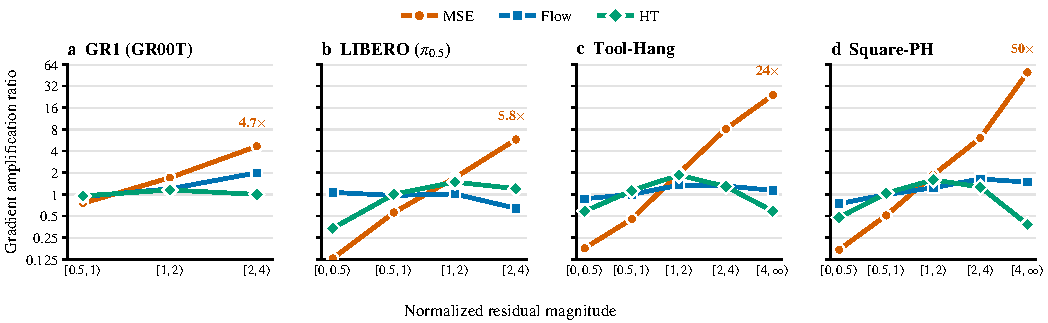
\includegraphics[width=\textwidth]{analysis/paper/gradient_distribution/fig_gradient_distribution.pdf}
  \caption{\textbf{HT prevents large-residual samples from dominating the gradient.}
  For each dataset, we bin samples by the action residual of a converged Flow
  policy (its deployed sampler's chunk minus the demonstrated chunk). The x-axis is the
  per-sample action-chunk residual RMS normalized by the pooled residual RMS. For each
  objective we differentiate the per-sample loss with respect to the network output
  (the predicted chunk for MSE and HT, the predicted velocity for Flow) and record the
  squared gradient norm; the gradient amplification ratio is each bin's share of the
  total squared output-gradient mass divided by its share of the data. $1\times$
  denotes proportional allocation, values above one indicate amplification,
  and values below one indicate suppression.
  Under MSE, gradient amplification grows sharply with residual magnitude,
  reaching $4.7\times$ on GR1, $5.8\times$ on LIBERO, $24.1\times$ on
  Tool-Hang, and $49.7\times$ on Square. Flow and HT keep the largest-residual
  bins near proportional allocation. All objectives within a panel are
  evaluated on the same residuals. Flow averages eight $(t, x_0)$ draws with
  $x_0\sim\mathcal{N}(0,I)$ and $t$ from each model's training law; HT uses
  $\nu=2d$ with the scale fixed at the pooled residual RMS. Panels (c,d) exclude the
  binary gripper channel.}
  \label{fig:gradient-distribution}
\end{figure*}
